\begin{enumerate}
    \item \texttt{matrixTest}
    \begin{itemize}
        \item Use the \texttt{listings} package to include your \texttt{matrixTest} output in the pdf.
        \item For each bug, use the \texttt{listings} package to display the original line of code with the error, as well as the fix.  Describe the error.            
    \end{itemize}
    \textbf{ANSWER:} \lstinputlisting[language={}]{gdbOutput.txt}
    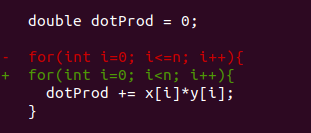
\includegraphics[width=0.5\textwidth]{Bug1.png} \newline
    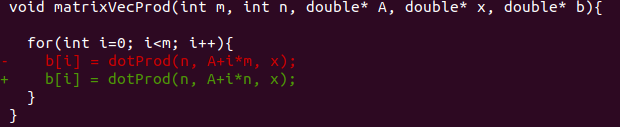
\includegraphics[width=\textwidth]{Bug3.png} \newline
    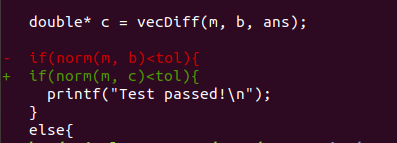
\includegraphics[width=0.5\textwidth]{Bug4.png} \newline
    The for loop has an equals sign as a parameter but there shouldn't be one because it's accessing unallocated areas of an array. \newline
    The formula to calculate the dot product was incorrect; C is a row ordered language so n should be used not m. \newline
    When testing the norm, b was used instead of c. I knew c should have been used because c was used for the same test statement further up in the file. Plus, c was defined but not used for anything within its scope.

    \item \texttt{fibonacci}
    \begin{itemize}
        \item Use the \texttt{listings} package to include your \texttt{fibonacci} output in the pdf.
        \item For each bug, use the \texttt{listings} package to display the original line of code with the error, as well as the fix.  Describe the error.
    \end{itemize}
    \textbf{ANSWER:} \lstinputlisting[language={}]{fibOutput.txt}
    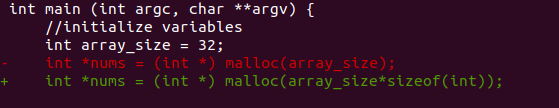
\includegraphics[width=\textwidth]{Bug5.png}
    The memory wasn't allocated right, we forgot to multiply by the size of an int when instantiating the array.

    \item \texttt{pascal}
    \begin{itemize}
        \item Use the \texttt{listings} package to include your \texttt{pascal} output in the pdf.
        \item For each bug, use the \texttt{listings} package to display the original line of code with the error, as well as the fix.  Describe the error.
    \end{itemize}
    \textbf{ANSWER:}
    \lstinputlisting[basicstyle=\tiny, language={}]{pasOutput.txt}
    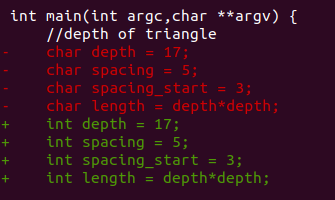
\includegraphics[width=0.7\textwidth]{Bug6.png} \newline
    The values were created as a char, not an int.

    \item \texttt{array\_sum}
    \begin{itemize}
        \item Use the \texttt{listings} package to include your \texttt{array\_sum} output in the pdf.
        \item For each bug, use the \texttt{listings} package to display the original line of code with the error, as well as the fix.  Describe the error.
    \end{itemize}
    \textbf{ANSWER:} \lstinputlisting[language={}]{sumOutput.txt}
    No bugs found.

    \item \texttt{rotate\_vector}
    \begin{itemize}
        \item Use the \texttt{listings} package to include your \texttt{rotate\_vector} output in the pdf.
        \item For each bug, use the \texttt{listings} package to display the original line of code with the error, as well as the fix.  Describe the error.
    \end{itemize}
    \textbf{ANSWER:} \lstinputlisting[language={}]{rotOutput.txt}
    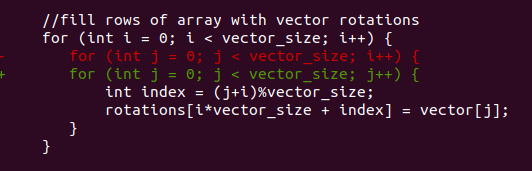
\includegraphics[width=\textwidth]{Bug2.png}
    When filling the rows of array with vector rotations, the nested for loop incremented i instead of j, so I changed it from i++ to j++.
    
\end{enumerate}
